\documentclass{beamer}

% There are many different themes available for Beamer. A comprehensive
% list with examples is given here:
% http://deic.uab.es/~iblanes/beamer_gallery/index_by_theme.html
% You can uncomment the themes below if you would like to use a different
% one:
%\usetheme{AnnArbor}
%\usetheme{Antibes}
%\usetheme{Bergen}
%\usetheme{Berkeley}
%\usetheme{Berlin}
%\usetheme{Boadilla}
%\usetheme{boxes}
%\usetheme{CambridgeUS}
%\usetheme{Copenhagen}
%\usetheme{Darmstadt}
%\usetheme{default}
%\usetheme{Frankfurt}
%\usetheme{Goettingen}
%\usetheme{Hannover}
%\usetheme{Ilmenau}
%\usetheme{JuanLesPins}
%\usetheme{Luebeck}
\usetheme{Madrid}
%\usetheme{Malmoe}
%\usetheme{Marburg}
%\usetheme{Montpellier}
%\usetheme{PaloAlto}
%\usetheme{Pittsburgh}
%\usetheme{Rochester}
%\usetheme{Singapore}
%\usetheme{Szeged}
%\usetheme{Warsaw}

\usepackage{CJKutf8}
\usepackage{tikz}
\usetikzlibrary{shapes.geometric, arrows}

\tikzset{
	flowchartnode/.style = {minimum width=3cm, minimum height=1cm, text centered, draw=black},
	process/.style = {rectangle, flowchartnode, fill=orange!30},
	decision/.style = {diamond, flowchartnode, fill=green!30},
	io/.style = {trapezium, trapezium left angle=70, trapezium right angle=110, flowchartnode, fill=blue!30},
	line/.style = {draw, -latex'}
}

\let\thefootnote\relax\footnotetext{Footnotetext without footnote mark}
\newcommand{\RNum}[1]{\uppercase\expandafter{\romannumeral #1\relax}}
\newcommand{\tab}[1]{\hspace{.1\textwidth}\rlap{#1}}

\usepackage{caption}
\usepackage{tabu}
\usepackage{listings}
\usepackage{color}
 
\definecolor{codegreen}{rgb}{0,0.6,0}
\definecolor{codegray}{rgb}{0.5,0.5,0.5}
\definecolor{codepurple}{rgb}{0.58,0,0.82}
\definecolor{backcolour}{rgb}{0.95,0.95,0.92}
 
\lstdefinestyle{mystyle}{
    backgroundcolor=\color{backcolour},   
    commentstyle=\color{codegreen},
    keywordstyle=\color{magenta},
    numberstyle=\tiny\color{codegray},
    stringstyle=\color{codepurple},
    basicstyle=\footnotesize,
    breakatwhitespace=false,         
    breaklines=true,                 
    captionpos=b,                    
    keepspaces=true,                 
    numbers=left,                    
    numbersep=5pt,                  
    showspaces=false,                
    showstringspaces=false,
    showtabs=false,                  
    tabsize=2
}

\lstset{style=mystyle}

\graphicspath{{fig/}}

%First page
\title[Progress Report]{Title need to change}

\author[Wei-Chih Chien]{Advicer : Gwan-Hwan Hwang\\ Student : Wei-Chih Chien}

\institute[NTNU CSIE CCLAB]{NTNU CSIE CCLAB}

\date{2015.10.29}

\AtBeginSection[]
{
  \begin{frame}<beamer>{Outline}
    \tableofcontents[currentsection]
  \end{frame}
}

% Let's get started
\begin{document}
\begin{CJK}{UTF8}{bkai}
\begin{frame}
  \titlepage
\end{frame}

\begin{frame}{Outline}
  \tableofcontents
\end{frame}

\section{Scenario}
\begin{frame}{Scenario}{Why Real-time Auditing?}
	\begin{center}
	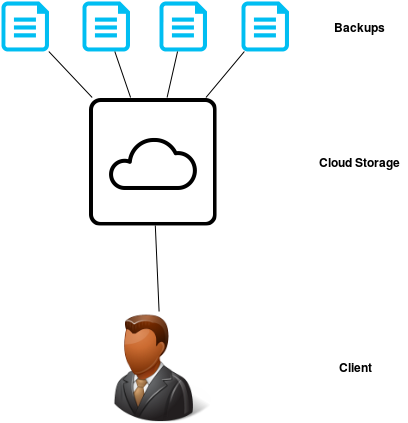
\includegraphics[width=.4\textwidth]{Scenario1.png}
	\end{center}
\end{frame}

\begin{frame}{Scenario (CON'T)}{Why Real-time Auditing?}
	\begin{minipage}{.49\hsize}
	\begin{center}
	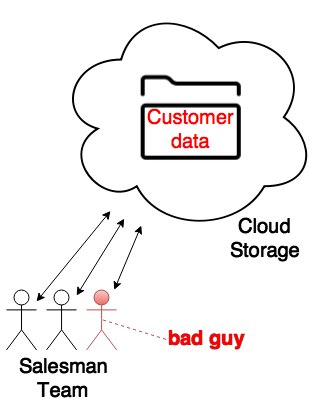
\includegraphics[width=.75\textwidth]{Scenario2.png}
	\end{center}
	\end{minipage}
	\pause
	\begin{minipage}{.49\hsize}
	\begin{center}
	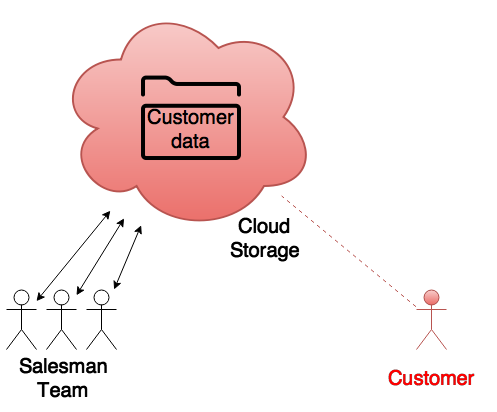
\includegraphics[width=.95\textwidth]{Scenario3.png}
	\end{center}
	\end{minipage}
\end{frame}

\section{Real-time Auditing Schemes}
\subsection{\small{Intuitive Method}}
\begin{frame}{Intuitive Method}
	\begin{center}
	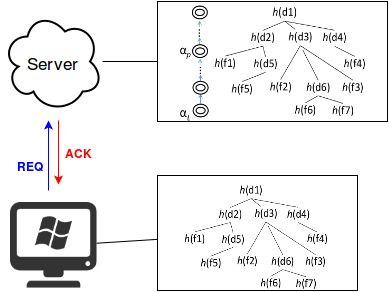
\includegraphics[width=.7\textwidth]{intuitive.png}
	\end{center}
\end{frame}

\subsection{\small{Instant Auditing of Cloud Storage Access by Cache Partial Merkle tree}}
\begin{frame}{\normalsize{Instant Auditing of Cloud Storage Access by Cache Partial Merkle tree}}
{\tiny{2014 IEEE 6th International Conference on Cloud Computing Technology and Science}}
	\begin{center}
	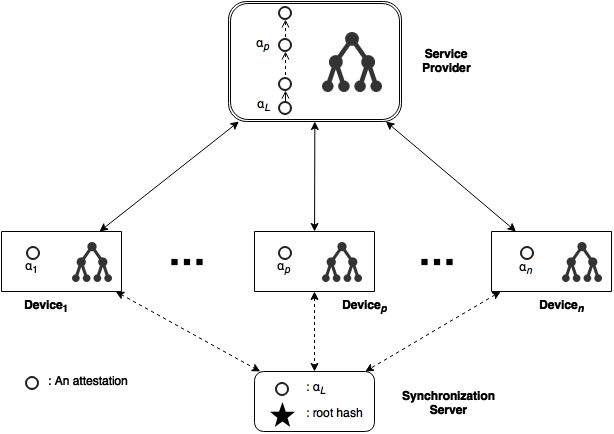
\includegraphics[width=.8\textwidth]{wei_shian.png}
	\end{center}
	\alert{Worst-case : 累積大量未更新的動作造成系統緩慢}
\end{frame}

\subsection{\small{My Method}}
\begin{frame}{My Method}
	\begin{center}
	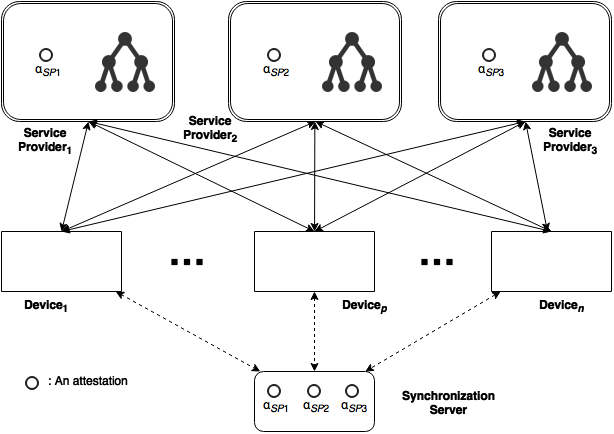
\includegraphics[width=.8\textwidth]{wei_chih.png}
	\end{center}
	\color{blue} Assumption: $\text{同時有k個server上同一file出問題的機率} \approx 0$
\end{frame}

\begin{frame}{Comparison}
	\begin{itemize}
		\item Pros
			\begin{enumerate}
				\item Service Provider 不用累積證據
				\item Client 不用佔用空間儲存證據
				\item 資料有多份備份
				\item 花費較少的時間更新到最新的狀態
			\end{enumerate}
		\item Cons
			\begin{enumerate}
				\item 硬體成本較高
				\item 需要處理多份 Response
			\end{enumerate}
	\end{itemize}
\end{frame}

\section{Protocol Detail}
\subsection{Flowchart}
\begin{frame}{Flowchart}
	\begin{center}
	\resizebox{!}{.6\textwidth}
	{%
		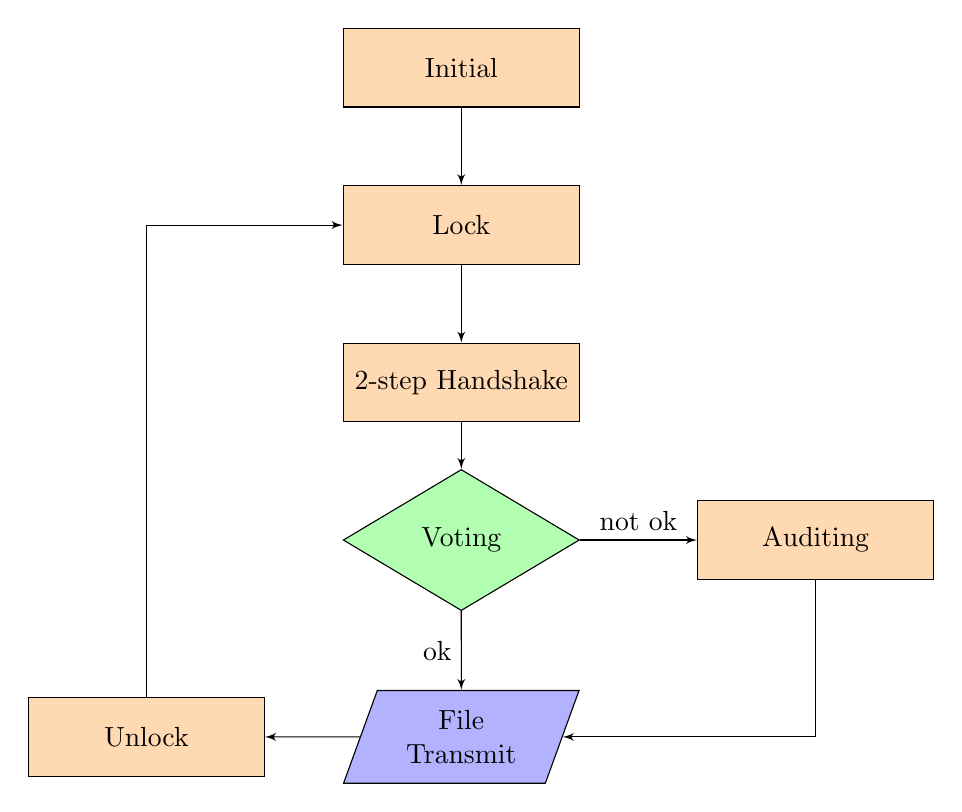
\begin{tikzpicture}[node distance=2cm]
		%定义流程图具体形状
		\node (init) [process] {Initial};
		\node (lock) [process, below of=init] {Lock};
		\node (twostep) [process, below of=lock] {2-step Handshake};
		\node (voting) [decision, below of=twostep] {Voting};
		\node (update) [io, below of=voting, align=center, yshift=-0.5cm] {File \\ Transmit};
		\node (auditing) [process, right of=voting, xshift=2.5cm] {Auditing};
		\node (unlock) [process, left of=update, xshift=-2cm] {Unlock};

		%连接具体形状
		\path [line](init) -- (lock);
		\path [line](lock) -- (twostep);
		\path [line](twostep) -- (voting);
		\path [line](voting) -- node[anchor=east] {ok} (update);
		\path [line](voting) -- node[anchor=south] {not ok} (auditing);
		\path [line](auditing) |- (update);
		\path [line](update) -- (unlock);
		\path [line](unlock) |- (lock);
		\end{tikzpicture}%
	}
	\end{center}
\end{frame}

\subsection{Initial}
\begin{frame}{Initial}
	\alert{File $\rightarrow$ Merkle Tree}\\
	\begin{center}
	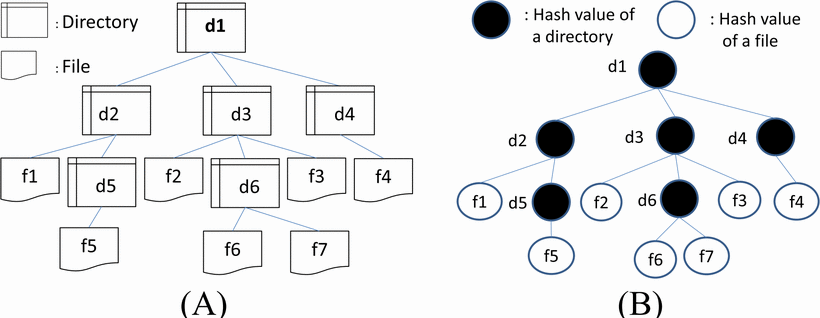
\includegraphics[width=.8\textwidth]{init.png}
	\end{center}
\end{frame}

\subsection{Read}
\begin{frame}{READ}{\RNum{1}. 2-step Handshake \& Voting}
	\begin{center}
	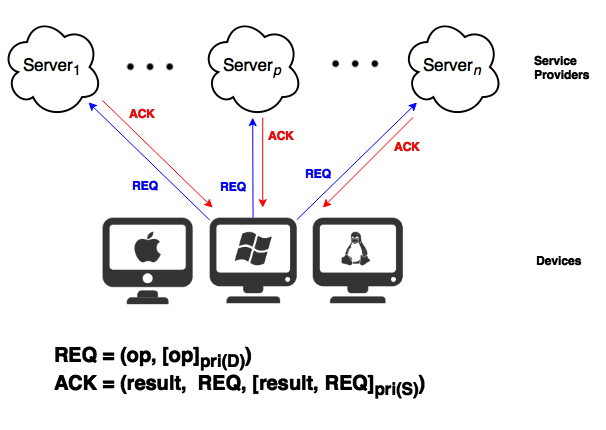
\includegraphics[width=.8\textwidth]{Read1.png}
	\end{center}
\end{frame}

\begin{frame}{READ}{\RNum{2}. Download}
	\begin{center}
	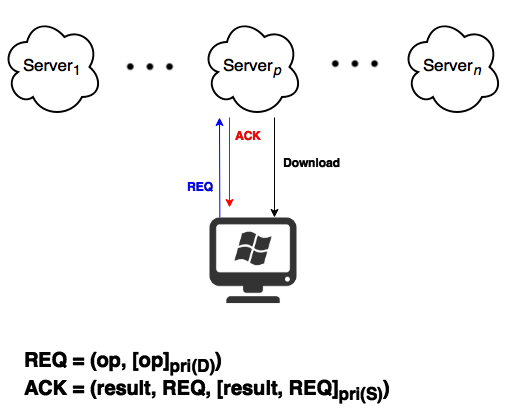
\includegraphics[width=.65\textwidth]{Read2.png}
	\end{center}
\end{frame}

\subsection{Write}
\begin{frame}{WRITE}{\RNum{1}. Upload}
	\begin{center}
	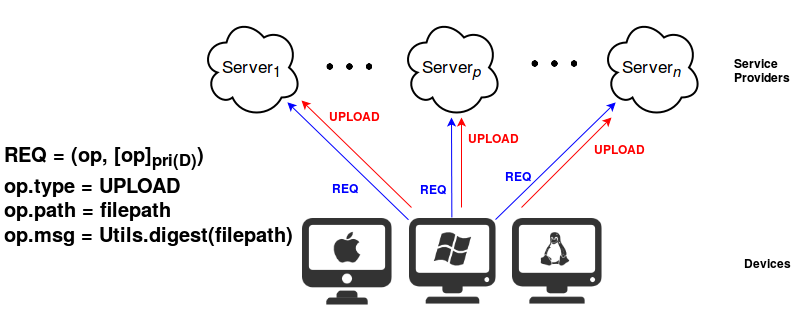
\includegraphics[width=.8\textwidth]{Write1.png}
	\end{center}
\end{frame}

\begin{frame}{WRITE}{\RNum{2}. Update Merkle Tree}
	\begin{center}
	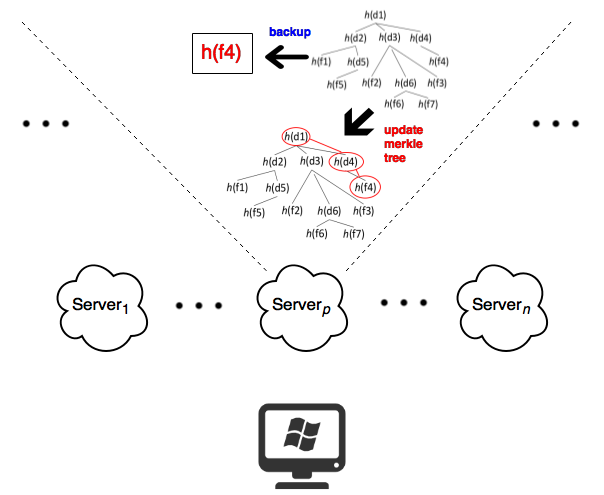
\includegraphics[width=.65\textwidth]{Write2.png}
	\end{center}
\end{frame}

\begin{frame}{WRITE}{\RNum{3}. Voting}
	\begin{center}
	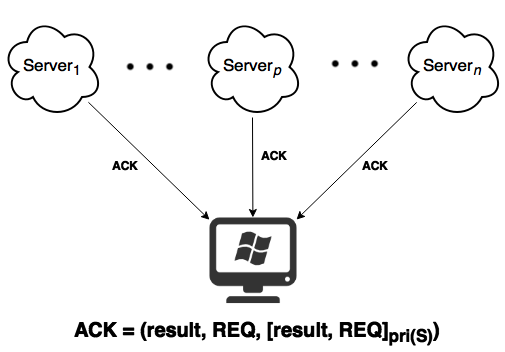
\includegraphics[width=.7\textwidth]{Write3.png}
	\end{center}
\end{frame}

\subsection{Audit}
\begin{frame}{AUDIT}
	\begin{enumerate}
		\item Device 向 \alert{Synchronization Server} 取得 Latest Ack.
		\item Device 再向 \alert{Service Provider} 取得 前一版本的 Merkle Tree.
		\item 使用 Step \RNum{1}. 的 Ack 包含的檔案 Hash 值\\
			  來更新 Step \RNum{2}. 的 Merkle Tree.
			  \begin{center}
			  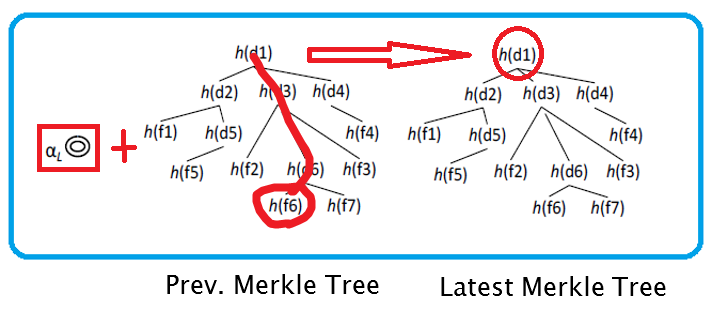
\includegraphics[width=.7\textwidth]{auditing.png}
			  \end{center}
		\item 比較 Device 自己算出的 Roothash 值是否和 Server 提供的相同.
	\end{enumerate}
\end{frame}

\section{Experimental Results}
\begin{frame}{Create Merkle Tree}
	\begin{center}
	Do it again.\\
	\begin{tabu}{cccc}
	\rowfont{\color{blue} \scriptsize} {Account A} & {666 MB}  & {42 files}     & {6 directories}    \\
	\rowfont{\color{blue} \scriptsize} {Account B} & {34 MB}   & {54192 files}  & {188 directories}  \\
	\rowfont{\color{blue} \scriptsize} {Account C} & {6.54 GB} & {58484 files}  & {1718 directories} \\
	\rowfont{\color{blue} \scriptsize} {Account D} & {20.6 GB} & {175389 files} & {5154 directories} \\
	\end{tabu}
	\end{center}
	\begin{table}[]
	\centering
	\captionsetup{justification=centering}
	\caption{\tiny TIMES REQUIRED TO GENERATE THE ROOT HASH FROM NOT-HASHED FILES (IN SECONDS)}
	\begin{tabular}{|c|c|c|c|}
	\hline
	{\bf Account} & {\bf Senior}  & {\bf My}      & {\bf MerkleTree Size} \\ \hline
	{\bf A}       & {\it 3.404}   & {\it 3.645}   & {3.74 KB}             \\ \hline
	{\bf B}       & {\it 16.618}  & {\it 7.669}   & {3.77 MB}             \\ \hline
	{\bf C}       & {\it 229.351} & {\it 242.198} & {4.30 MB}             \\ \hline
	{\bf D}       & {\it }        & {\it 815.408} & {12.9 MB}             \\ \hline
	\end{tabular}\\
	\end{table}
\end{frame}
\begin{frame}{Operation Processing Time}
	\begin{table}[]
	\makebox[0pt][c]{\parbox{\textwidth}{%
	\begin{minipage}{.47\hsize}
	\captionsetup{justification=centering}
	\caption{DOWNLOAD TIME (ms)}
	\begin{tabu}{|c|c|c|}
	\hline
	\rowfont{\color{blue}} {\bf Account} & {\bf 100 times} & {\bf Audit$^*$} \\ \hline
	\rowfont{\color{blue}} {\bf A}       & {\it 4635}      & {\it 34 + 0}    \\ \hline
	\rowfont{\color{blue}} {\bf B}       & {\it 4660}      & {\it 33 + 0}    \\ \hline
	\rowfont{\color{blue}} {\bf C}       & {\it 5429}      & {\it 31 + 0}    \\ \hline
	\rowfont{\color{blue}} {\bf D}       & {\it 5554}      & {\it 31 + 0}    \\ \hline
	\end{tabu}
	\end{minipage}
	\begin{minipage}{.53\hsize}
	\captionsetup{justification=centering}
	\caption{UPLOAD TIME (ms)}
	\begin{tabular}{|c|c|c|}
	\hline
	{\bf Account} & {\bf 100 times} & {\bf Audit$^*$}   \\ \hline
	{\bf A}       & {\it 4322}      & {\it 41  + 7}     \\ \hline
	{\bf B}       & {\it 5643}      & {\it 421 + 997}   \\ \hline
	{\bf C}       & {\it 9236}      & {\it 421 + 2621}  \\ \hline
	{\bf D}       & {\it 11466}     & {\it 1263 + 8085} \\ \hline
	\end{tabular}
	\end{minipage}
	}}
	\footnote{* download attestations time + audit time}
	\end{table}	
\end{frame}

\section{Schedules}
\begin{frame}{Schedules}
	\begin{enumerate}
	{\color{blue}
	\item My Method Finished.
		\begin{itemize}
			\item Merkle Tree Implements.
			\item Operation Handle (Read, Write and Audit).
			\item File Transmit.
			\item Object Transmit (Serialization).
			\item Synchronization Server Implements.
		\end{itemize}
	\item Wei-Shian's Method Finished.}
		\begin{itemize}
			\item Attestation Chain Implements.
		\end{itemize}
	\item \alert{Design Different Experiments.}
	\end{enumerate}
\end{frame}

\begin{frame}
	\begin{center}
	
\includegraphics[width=\textwidth]{thank_you.jpg}
	\end{center}	
\end{frame}
\end{CJK}
\end{document}
